\documentclass{beamer}
\let\Tiny=\tiny %to avoid warnings related to font size and beamer 
\usetheme{Amsterdam}
\usecolortheme{dolphin}

\usepackage{graphicx}
\usepackage{comment}

\usepackage[style=numeric-comp,backend=bibtex]{biblatex}
\addbibresource{sources}

%reduce font size of footnotes
\let\oldfootnotesize\footnotesize
\renewcommand*{\footnotesize}{\oldfootnotesize\tiny}

\newcommand\fR[1]{\textcolor{red!80!black}{\textbf{#1}}}
\newcommand\fB[1]{\textcolor{blue!80!black}{\textbf{#1}}}
\newcommand\fG[1]{\textcolor{green!70!black}{\textbf{#1}}}

%---------------------------------------------------------------------
%Front matter
%---------------------------------------------------------------------
\title{INSPIRE}
\subtitle{The Insieme Parallel Intermediate Representation}
\author{Martin Kalany}
\institute
{
  Graduate student in Computer Science\\
  Vienna University of Technology\\
}
\date{\today}

\begin{document}
\maketitle

\section{Standards}
\begin{frame}
\frametitle{Some standards for parallel programming}
\begin{itemize}
\item \fB{MPI} message passing, distributed memory
\item \fB{OpenMP} shared memory
\item \fB{OpenCL} across heterogenous platforms

\bigskip
\item \fB{Hybrid architecures} MPI/OpenMP, OpenMP/OpenCL,...
\end{itemize}
\end{frame}

\section{Problem}
\begin{frame}
\frametitle{The problem}

\fB{Compiler view:} Just another library used by a sequential host language. Parallel constructs \fR{not native} constructs within most programming languages.

\bigskip\pause
\fR{Parallel control flow} remains \fR{hidden} in library calls embedded in sequential IR\footnote{IR: intermediate representation}.

\bigskip\pause
Sequential IR \fR{cannot represent parallelism} appropriately and explicitly.

\bigskip\pause
$\Rightarrow$ \fR{Optimizations} of parallel constructs \fR{not possible} for compiler. 
\end{frame}

\section{Concepts}
\begin{frame}
\frametitle{The idea}
\fB{INSPIRE}~\cite{JordanPTKF13}  is a
\begin{itemize}
\item unified,
\item parallel,
\item high-level,
\item language independent IR

\smallskip
modelling parallel constructs explicitly.
\end{itemize}
\bigskip\pause
\fG{Goal:} Make parallel control flow available to compiler.
\end{frame}

\begin{frame}
\frametitle{Some concepts}
INSPIRE is based on recursively nested thread groups

\bigskip
\fB{Thread}: Arbitrary entity capable of preocessing sequential control flow (e.g., OS and OpenMP threads, MPI Processes, OpenCL work items,...)

\bigskip
\fB{Job}: executed cooperatively by each thread in a group

\bigskip
\fB{Spawn}: A thread may spawn a new thread group

\bigskip
\fB{Merge} and \fB{MergeAll}: Block until referenced thread group finished 
\end{frame}

\begin{frame}
\frametitle{Concepts cont.}
\fB{Inter-Thread Communication}
\begin{itemize}
\item \fB{pfor}: distribute work (e.g., \texttt{parallel for} in OpenMP)
\item \fB{redistribute}: data redistribution (e.g., \texttt{scatter} and \texttt{gather} in MPI). Collects contributions from all threads; generic function to select what piece of information available to local thread.
\item \fB{channels}: Point to point communication
\end{itemize}

\bigskip
\texttt{pfor} and \texttt{redistribute} are reduction operations. %The latter is a blocking operation.

\bigskip\pause
Generic \fB{atomic} operator: conditional, protected assignment to single memory location.
\end{frame}

\begin{frame}
\frametitle{IR Structure}

\begin{center}
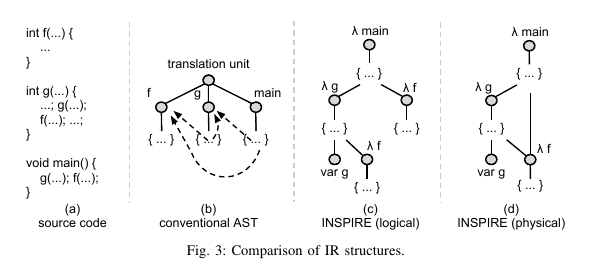
\includegraphics[width=250pt]{structure}
\end{center}

\begin{itemize}
\item Does not reflect structure of translation units. 
%(root is usually the file)

\item Instead models actual execution as single expression. 
%(root element is typically the main function)

\item Function calls mapped at call site. 
%(i.e., different calls represented by different nodes.  No global context required, context sensitive optimization possible and simple since node specific)
\end{itemize}
\end{frame}


%---------------------------------------------------------------------
%bibliography
%---------------------------------------------------------------------
\begin{frame}[allowframebreaks]
\frametitle<presentation>{Literature}    
\printbibliography
\end{frame} 	 
\end{document}